\paragraph[QuizziPedia::Front-End::ModelViews\\::QuestionnaireDetailsModelView]{QuizziPedia::Front-End::ModelViews::QuestionnaireDetailsModelView}
	
	\label{QuizziPedia::Front-End::ModelViews::QuestionnaireDetailsModelView}
	
	\begin{figure}[ht]
		\centering
		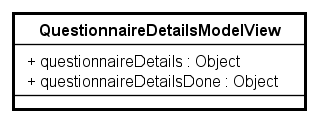
\includegraphics[scale=0.5,keepaspectratio]{UML/Classi/Front-End/QuizziPedia_Front-end_ModelView_QuestionnaireDetailsModelView.png}
		\caption{QuizziPedia::Front-End::ModelViews::QuestionnaireDetailsModelView}
	\end{figure} \FloatBarrier
	
	\begin{itemize}
		\item \textbf{Descrizione}: classe di tipo modelview la cui istanziazione è contenuta all'interno della variabile di ambiente \texttt{\$scope} di \textit{Angular\ped{G}}. All'interno di essa sono presenti le variabili e i metodi necessari per il \textit{Two-Way Data-Binding\ped{G}} tra la \textit{view\ped{G}} \texttt{UserView} e il \textit{controller\ped{G}} \texttt{QuestionnaireDetailsController};
		\item \textbf{Utilizzo}: viene utilizzata per effettuare il \textit{Two-Way Data-Binding\ped{G}} tra la \textit{view\ped{G}} \texttt{UserView} e il \textit{controller\ped{G}} \texttt{QuestionnaireDetailsController} rendendo disponibili variabili e metodi;
		\item \textbf{Relazioni con altre classi}: 
		\begin{itemize}
			\item \textbf{OUT \texttt{QuestionnaireDetailsDirective}}: rappresenta il componente grafico che permette all'utente di visualizzare la lista di questionari che può compilare;
			\item \textbf{OUT \texttt{QuestionnaireDetailsDoneDirective}}: rappresenta il componente grafico che permette all'utente di visualizzare la lista di questionari che ha già compilato e di conseguenza vederne le valutazioni;
			\item \textbf{OUT \texttt{QuestionnaireDetailsController}}: questa classe permette di gestire i dettagli di un questionario.
		\end{itemize}
		\item \textbf{Attributi}: 
		\begin{itemize}
			\item \texttt{+ questionnaireDetails: Object} \\ Oggetto contenente i seguenti campi dati:
			\begin{itemize}
				\item \texttt{name: String}\\ Nome del questionario;
				\item \texttt{author: String}\\ Autore del questionario;
				\item \texttt{topic: String}\\ Argomento del questionario;
				\item \texttt{keywords: Array<String>}\\ Parole chiave del questionario.
			\end{itemize}
			\item \texttt{+ questionnaireDetailsDone: Object} \\ Oggetto contenente i seguenti campi dati:
			\begin{itemize}
				\item \texttt{name: String}\\ Nome del questionario;
				\item \texttt{author: String}\\ Autore del questionario;
				\item \texttt{topic: String}\\ Argomento del questionario;
				\item \texttt{keywords: Array<String>}\\ Parole chiave del questionario;
				\item \texttt{judgement: Number} \\ Campo che indica il risultato del questionario.
			\end{itemize}
		\end{itemize}
	\end{itemize}
	
		